\section{Referencial teórico}

\begin{frame}[allowframebreaks]{Acústica}  
  \begin{figure}[t]
    \centering
    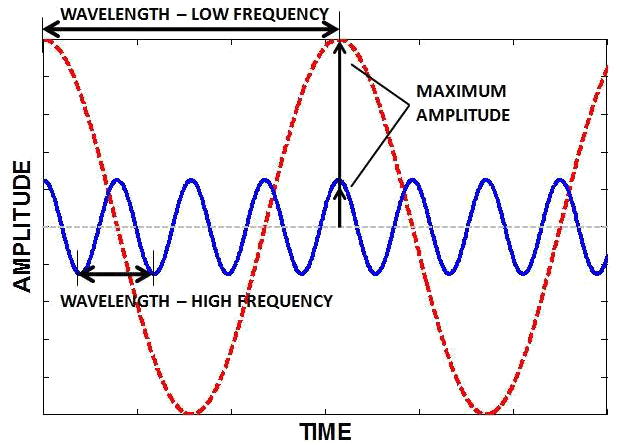
\includegraphics[height=\dimexpr10\textheight/16\relax]{figuras/wave}
    \caption{Frequência e intensidade sonora}
  \end{figure}
	\begin{center}
	\tiny \textbf{Fonte:} \url{http://wingchunus.com/how-fast-should-you-punch/}
	\end{center}
%\end{frame}

%--------------------------------------------------------------%

%\begin{frame}{Acústica}  
  \begin{figure}[t]
    \centering
    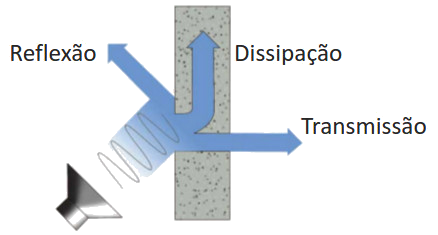
\includegraphics[height=\dimexpr8\textheight/14\relax]{figuras/reflexao}
    \caption{Reflexão}
  \end{figure}
	\begin{center}
	\tiny \textbf{Fonte:} \url{http://www.metalica.com.br/desempenho-acusticos-em-sistemas-drywall}
	\end{center}
%\end{frame}

%--------------------------------------------------------------%

%\begin{frame}{Acústica}
Intensidade sonora:
\begin{large}
\[I_{0} = 10^{-12}~W/m^{2}\]
\[I_{max} = 1~W/m^{2}\]
\end{large}

Nível de intensidade sonora (Decibel):
{\large \[d\beta = 10 \log \frac{I}{I_{0}}\]}
Tempo de reverberação (RT60): tempo em que o nível de intensidade sonora no ambiente cai em 60 dB.
\end{frame}

%--------------------------------------------------------------%

\begin{frame}{Simulação}
Simulação é a representação de um processo do mundo real para um ambiente controlado onde se pode estudar o comportamento do mesmo, sob diversas condições, sem riscos físicos e/ou grandes custos envolvidos \cite{torga}.
\linebreak
\linebreak
\begin{center}
Simulação x Simulação Computacional
\end{center}
\end{frame}

%--------------------------------------------------------------%

\begin{frame}{Simulação acústica}
Um dos modelo de representação acústica de ambientes fechados é \textbf{acústica geométrica de salas}, onde o conceito de onda sonora é substituído pelo conceito de raio sonoro \cite{torres}.

  \begin{figure}[t]
    \centering
    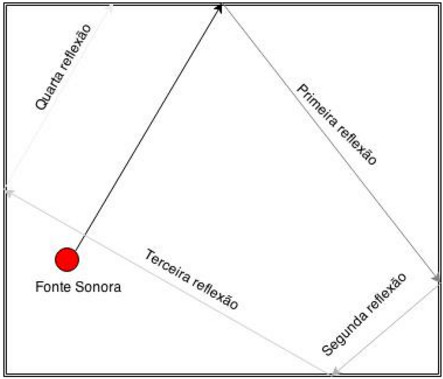
\includegraphics[height=\dimexpr7\textheight/14\relax]{figuras/reflexoes}
    \caption{Reflexão dos raios sonoros}
  \end{figure}
  
\end{frame}